At the simplest level of abstraction, a Generative Adversarial Network (GAN)~\cite{goodfellow2014generative} places a Generator $G$ and a Discriminator $D$ against one another in a two-player minimax game.
$G$ looks to generate images of probability distribution $p(g)$ to match the training images of probability distribution $p(r)$ as closely as possible.
This is done by attempting to transform $p(g)$ towards $p(r)$ by minimising a given distance metric.

The Deep Convolutional Generative Adversarial Network (DCGAN)~\cite{radford2015unsupervised} improves on the GAN by replacing fully-connected layers with convolution layers.
The idea is that these convolution kernels can learn spacial features matching the distribution of the input dataset.
As with the original DCGAN implementation, the generator and discriminator consist of equivalent but opposite operations (with 2D convolutions in the discriminator and 2D transposed convolutions in the generator).
For the generator, this consists of taking an $n_l \times 1 \times 1$ latent representation and transpose-convolving (thus unscaling) through five layers to a $3 \times 64 \times 64$ image representation.
The discriminator performs the opposite, taking the input image from a $3 \times 64 \times 64$ image representation to a scalar discrimination value (representing whether the discriminator thinks the image is from the training set or not).

Some common distance metrics include Kullback-Leibler (KL) divergence, and its extension Jensen-Shannon (JS) divergence.
While these can perform well under well-tuned hyperparameters and a more simple dataset, they both suffer from gradient instability.

At its core, this method consists of a modified version of a Wasserstein GAN~\cite{arjovsky2017wasserstein} (WGAN).
WGANs look to alleviate the training instability inherent within KL and JS using the Wasserstein distance metric.
This is given by
\begin{equation}
    \max_{\norm{f}_L \leq 1} \E_{\vx \sim p_{\textrm{data}}}[f(\vx)] - \E_{\vx \sim p_{\textrm{gen}}}[f(\vx)]
    \label{eq:wasserstein}
\end{equation}

Where $p_{\textrm{data}}$ represents real images and $p_{\textrm{gen}}$ represents images generated from random noise.

The idea here is that the discriminator tries to maximise the difference between $\E_{\vx \sim p_{\textrm{data}}}[f(\vx)]$ and $\E_{\vx \sim p_{\textrm{gen}}}[f(\vx)]$ whereas the generator wants to minimise it.

In terms of implementation, at the end of the forward pass for the discriminator, the 0--1 normalising sigmoid function $\sigma{x}$ is removed.
Because it no longer outputs the likelihood of the image being fake, the discriminator is renamed to the 'Critic'.
As an added advantage, the critic's loss value now correlates with the convergence of the generator.
Additionally, the critic is trained more than the generator (five times per generator training step).
Figure~\ref{fig:architecture} shows a diagram demonstrating the inputs, outputs and architecture of the WGAN\@.

While WGANs improve stability (and attempt to prevent mode collapse), they do this at the cost of having potentially longer training times.
This is partly down the need to satisfy the Lipschitz constraint (the $\max_{\norm{f}_L \leq 1}$ term in Equation~\ref{eq:wasserstein}), which the original paper proposes be done by clipping all the weights to lie within a constant range around zero.
It also recognises that depending on the clipping parameter, a small value may lead to vanishing gradients whereas a large value may dramatically increase training times (as weights may take a while to reach their limit).
~\cite{gulrajani2017improved} looks to remedy this by proposing a WGAN with Gradient Penalty (GP) - a different way to satisfy the Lipschitz constraint.
This works by adding a GP term to the original WGAN loss as follows.
\begin{equation}
    \E_{\vx \sim p_{\textrm{gen}}}[f(\vx)] - \E_{\vx \sim p_{\textrm{real}}}[f(\vx)]
    + \lambda \E_{\hat{\vx} \sim p_{\hat{\vx}}}[(\norm{\nabla_{\hat{\vx}} D(\hat{\vx})}_2 - 1)^2]
    \label{eq:wasserstein-gp}
\end{equation}

Where $\lambda$ is the penalty coefficient which determines how much weight is given to the GP\@, and $p_{\hat{\vx}}$ is the distribution over the interpolated samples $\epsilon \vx + (1 - \epsilon) \tilde{\vx}$ between real image $\vx$ and randomly generated image $\widetilde{\vx}$ for randomly sampled $\epsilon \in u[0, 1]$.
Notice the first two terms have switched, this now means that its negation is used as the loss.

\begin{figure}[h]
    \centering
    \caption{WGAN architecture}
    \label{fig:architecture}
    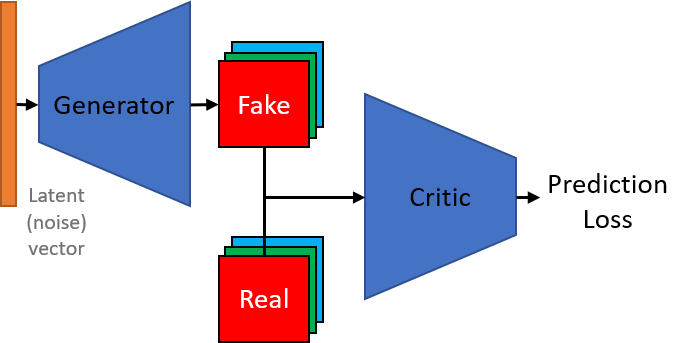
\includegraphics[width=0.5\textwidth]{figures/architecture}
\end{figure}

The hyperparameters are shown in Table~\ref{tab:1} and are generally kept the same as used in their respective original papers and implementations.
\begin{table}[t]
    \centering
    \caption{Hyperparameters for WGAN with GP}
    \label{tab:1}
    \begin{tabular}{l l}
        HYPERPARAMETER               & VALUE \\ [0.5ex]
        \hline
        Adam learning rate           & $0.0001$       \\
        Adam $\beta_1$               & $0.0$          \\
        Adam $\beta_2$               & $0.9$          \\
        Mini-batch size              & $64$           \\
        Input image channels         & $3$            \\
        Input image size             & $64 \times 64$ \\
        Latent features              & $100$          \\
        Critic base features         & $16$           \\
        Generator base features      & $16$           \\
        Critic iterations            & $5$            \\
        Gradient penalty $\lambda{}$ & $10$           \\
        Epochs                       & $500$ \\ [1ex]
    \end{tabular}
\end{table}

To achieve Pegasus-like outputs, the WGAN is trained on the CIFAR-10~\cite{krizhevsky2009cifar10} and STL-10~\cite{coates2011stl10} datasets.
As part of pre-processing, the images are resized to 64x64 pixels and normalised (as required for WGAN convergence).
Finally, all images except those labeled as horses and birds are discarded.
Since WGANs prevent mode collapse, when trained randomly on both horses and birds, the resultant generated images should consist of a combination of horse and bird features.
This works on the hope that a subset of the convolutions will produce horse-like features and another subset will produce bird-like features (wings being the most desirable).
Because of this, it is expected that most outputs will not look like Pegasus, with potentially only a few per 64-batch matching the criteria.
